\documentclass{article}
\newcommand{\exptitle}{Neutron Irradiation}
\newcommand{\course}{PHYS3112 - Experimental and Computational Physics}

\usepackage{graphicx}
\usepackage{pgf}
\usepackage{lmodern}
\usepackage{import}
\usepackage{booktabs}
\usepackage{tabu}
\usepackage{float}
\usepackage[hidelinks]{hyperref}
\usepackage{amsmath}
\usepackage{amsfonts}
\usepackage[margin=1in]{geometry}
\usepackage{pythonhighlight}
\usepackage[toc]{appendix}
\usepackage{float}
\usepackage{placeins}
\usepackage{natbib}
\usepackage{lmodern}
\usepackage{subfig}
\usepackage[utf8]{inputenc}
\usepackage[T1]{fontenc}
\usepackage{upgreek}
\usepackage{chemmacros}
\usepackage{braket}
\usepackage{newpxtext,newpxmath}
\usepackage{tikz}

\DeclareMathOperator{\sech}{sech}
\DeclareMathOperator{\cosech}{cosech}

\setlength{\parskip}{1em}
\setlength{\parindent}{0em}

\begin{document}

\begin{titlepage}
    \begin{center}
        \vspace*{7cm}

        \Huge
        \textbf{\exptitle}

        \vspace{0.5cm}
        \LARGE
        \course

        \vspace{1.5cm}

        \textbf{Toby Nguyen - z5416116}
    \end{center}
\end{titlepage}

\tableofcontents


\section{Introduction}
Neutron irradiation of elements is a good and useful tracer for detecting certain isotopes. This involves 
irradiating a sample with thermal neutrons to calculate the half life of the sample. This has many uses 
such as in industry, medicine and sciences. For example, Boron Neutron Capture Therapy (BNCT) is a cancer 
treatment that uses neutron irradiation to target and destroy cancerous tumours.

\section{Method}
\subsection{Equipment}
The neutron source in this experiment was a 20GBq americium-241 that was mixed with beryllium powder
and sealed in a stainless steel cylinder. The americium-241 would emit $\alpha$-particles which 
react with the beryllium to produce neutrons, based on the following process:
\begin{reaction}
    4^9Be + 2^4He -> 6^12C + 0^1n + Q
\end{reaction}

\begin{figure}
    \centering
    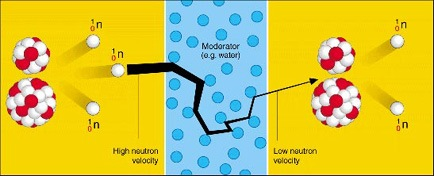
\includegraphics[width=0.8\textwidth]{../Figures/moderator.jpg}
    \caption{Example of water being used as a moderator to slow down neutron's kinetic energy}
    \label{fig:moderator}
\end{figure}

The paraffin moderating block slows down fast neutrons to thermal energies, acting as the neutron 
moderator. Neutron moderators are used to increase neutron and target nuclei interactions. Fast 
neutrons have too high energy to efficiently interact with the target nuclei whilst the thermal 
neutrons (Neutrons in thermal equilibrium with their surroundings) have much higher cross sections, 
increasing probability of interactions. The fast neutrons passing through the moderator will collide 
elastically with the moderator atoms, reducing their kinetic energy as seen in Figure \ref{fig:moderator}.

To count the radiation, a Geiger-Muller tube is used. When high energy particles or gamma radiation 
enters the tube to ionise the low pressure gas inside the tube, an electrical charge is sent out
to continue the count.

\subsection{Theory}
The decay rate of a nuclei is dependent on the number of nuclei present,

\begin{equation}
    -\frac{dn}{dt} = \lambda n
\end{equation}

where $\lambda$ is the decay constant. Integrating gives 

\begin{align}
    \int \frac{dn}{n} &= \int -\lambda dt \\
    \ln(n) &= -\lambda t + c \\
    n &= e^{-\lambda t + c}
\end{align}

If we set $t=0$, then c, the constant of integration represents the 
number of nuclei present initially, i.e $e^c = n_0$,

\begin{equation}
    n = n_0 e^{-\lambda t}.
    \label{eqn:n}
\end{equation}

Experimentally, we want to fit a log linear version of this graph,
so,

\begin{equation}
    \ln \left( \frac{n}{n_0} \right) = -\lambda t.
    \label{eqn:logn}
\end{equation}

The half life, $\tau_{1/2}$, is the time it takes for half the nuclei 
in the radioactive material to decay so $n=\frac{n_0}{2}$,

\begin{align}
    \frac{n_0}{2} &= n_0e^{-\lambda t } \\
    \frac{1}{2} &= e^{-\lambda t} \\
    \ln \left( \frac{1}{2} \right) &= -\lambda t \\ 
    \tau_{1/2} &= \frac{\ln(2)}{\lambda}
    \label{eqn:hl}
\end{align}

Rather than measuring $n$ or $\frac{dn}{dt}$, we will measure the 
count rate, $c$, which is proportional to the decay rate, $\lambda$,

\begin{equation}
    c = K\left(-\frac{dn}{dt}\right) = k\lambda n
\end{equation}

where K and k are some constants. To find these constants, consider 
a situation where some target nuclei $n_T$ are exposed to a flux of 
neutrons, $\phi$ per unit time. The probability of neutron capture or 
the neutrons interacting with the nuclei is based on the area of the 
nuclei, $\sigma$. Therefore, the rate of change of the product nuclei
is given by

\begin{equation}
    \frac{dn}{dt} = \phi \sigma n_T - \lambda n
\end{equation}

Integrating gives 

\begin{equation}
    n = \frac{\phi \sigma n_T}{\lambda} \left(1 - e^{-\lambda t} \right).
    \label{eqn:s}
\end{equation}

Note that when $t \gg \frac{1}{\lambda}$, the number of product nuclei 
saturates.

\subsection{Poisson Statistics}

The counting of neutrons over an interval of time can be represented as 
a Poisson distribution. This is because the counting events occur independently 
of each other and the events occur randomly in time, with the probability of 
a neutron count occuring in a small time interval being proportional to the 
length of that interval. Furthermore, the average rate of events is constant 
for any small interval of time $dt$. This allows us to model exponential decay, 
Equation \ref{eqn:n} and the saturation point, Equation \ref{eqn:s}, as Poisson 
processes. We are then able to find the probability of any $n$ number of counts 
in an interval of time,

\begin{equation}
    P(X=n) = \frac{\lambda^n e^{-\lambda}}{n!}
\end{equation}

where $\lambda$ represents the expected number of counts over an interval of time.
We will exploit the fact that the variance of the distribution is equal to the number 
of counts. Therefore the standard deviation of the total counting events for each 
measurement is given as,

\begin{equation}
    \sigma_{\text{random}} = \sqrt{n}
    \label{eqn:sigma}
\end{equation}

where n is the number of counts for the measurement. 

\section{Results and Analysis}
The error bars for all graphs were given by Equation \ref{eqn:sigma}. The uncertainty 
for each calculated value from using the fitted parameters are given by the covariance 
matrix produced the scipy.optimize.curvefit function.

\begin{figure} [H]
    \centering
    \subfloat[]{\scalebox{0.55}{\input{../Figures/exp1graph.pgf}}}
    \subfloat[]{\scalebox{0.55}{\input{../Figures/exp1graphl.pgf}}}
    \caption{(a) Left: Decay function, Equation \ref{eqn:n}, of the overnight Indium sample. 
    The count was done for as long as time was permitted, 
    i.e long enough to see an exponential curve rather than 
    a linear function. The counting interval was 600 seconds and left for 26 runs.
    The fitted curve using scipy.curvefit 
    has a $\lambda$ of 0.0002 and an initial count of 2178. We can use 
    Equation \ref{eqn:hl} to find the half life of Indium.
    (b) Right: Log linear function of the decay curve above, fitted to 
    a theoretical model found in Equation \ref{eqn:logn}. We find that 
    the gradient which corresponds to $-\lambda$ is equal to 0.0002 which 
    is the same as the figure on the left.}
    \label{fig:exp1}
\end{figure}

We can find the half life of Indium by using Equation \ref{eqn:hl},
with the value for $\lambda$ given as 0.0002 from Figure \ref{fig:exp1},

\begin{align}
    \tau_{1/2} &= \frac{\ln(2)}{\lambda} \\
    &= \frac{\ln(2)}{0.0002} \\
    &= 3466\text{ s} \\
    &= 57.7 \pm 0.8\text{ min}.
\end{align}

\begin{figure} [H]
    \centering
    \subfloat[]{\scalebox{0.55}{\input{../Figures/exp2graph.pgf}}}
    \subfloat[]{\scalebox{0.55}{\input{../Figures/exp2graphl.pgf}}}
    \caption{(a) Left: Graph displaying the count of 8 different Indium samples
    irradiated over various times: 10, 25, 40, 60, 90, 120, 150 and 180 
    minutes. The counting interval was 600 seconds for 1 run for each sample. 
    We expected to find a saturation point in which the count 
    levels out for an increasing irradiation time, which according to 
    the fitted curve lies approximately in the 3500 range. This saturation 
    point will occur when $t \gg \frac{1}{\lambda}$, using the $\lambda$ 
    value in the fitted curve will correspond to when the irradiated time 
    is greater than 44 seconds. (b) Right: Graph displaying count versus a transformed x axis so 
    that the gradient of the linear function corresponds to the constant
    factor in Equation \ref{eqn:s}, $\frac{\phi \sigma n_T}{\lambda}$.}
    \label{fig:exp2}
\end{figure}

We can calculate the saturation point by taking the ratio of $k$ to $\lambda$,

\begin{align}
    S &= \frac{k}{\lambda} \\
    &= \frac{81.9}{0.02} \\
    &= 3538 \pm 1816 \text{ counts.}
\end{align}

\begin{figure} [H]
    \centering
    \subfloat[]{\scalebox{0.55}{\input{../Figures/exp3graph.pgf}}}
    \subfloat[]{\scalebox{0.55}{\input{../Figures/exp3graphl.pgf}}}
    \caption{(a) Left: Decay function of silver over the last 5 minutes of the 
    7.5 minutes we recorded the counts over. Each counting interval 
    was 30 seconds, left for 15 runs. The graph above shows the last 
    10 runs. The fitted curve returns a $\lambda$ value of 0.0052.(b) Right:
    Log count vs time to produce a linear function. The solid blue lines 
    represent the fitted linear function for all 15 runs. The higher and 
    lower solid lines represent the upper and lower bound in the extrapolation, 
    found by using the $\Delta m$ and $\Delta b$ found in the covariance 
    matrix produced by scipy.optimize.curvefit. The dotted orange line is 
    the fitted curve for the last 10 runs, note the shallower gradient.
    }
    \label{fig:exp3}
\end{figure}

The half life of silver can be calculated using Equation \ref{eqn:hl}, with 
the parameter, $\lambda = 0.0052$, obtained from the Figure \ref{fig:exp3} 
above.

\begin{align}
    \tau_{1/2} &= \frac{\ln(2)}{\lambda} \\
    &= \frac{\ln(2)}{0.0052} \\
    &= 133.3 \text{ s}.
\end{align}

Comparing this to widely used accepted values for the half life of silver, 
we find that this silver sample corresponds to \ch{^{100}47Ag}. Extrapolating 
the curve fit back to zero time obtains us a lower bound of 6.77 and an upper bound 
of 7.05 with an estimated value of 6.91 from the curve of best fit. Transforming these 
log counts into initial counts will give us 872, 1001 and 1153 (rounded up).

\begin{figure} [H]
    \centering
    \scalebox{0.75}{\input{../Figures/exp4graph.pgf}}
    \caption{The count of each irradiated 'sandwich' of 2 shielding discs and 
    Indium. We find that unsurprisingly, no shield would produce the most counts 
    of neutron irradiation. From weakest to strongest shield would be lead, indium 
    and cadmium.}
    \label{fig:exp4graph}
\end{figure}

\begin{figure} [H]
    \centering
    \subfloat[]{\scalebox{0.55}{\input{../Figures/exp5graph.pgf}}}
    \subfloat[]{\scalebox{0.55}{\input{../Figures/exp5graph2.pgf}}}
    \caption{(a) Left: Decay function of copper. The copper was irradiated for 90 minutes 
    and the count was done every 60 seconds for 25 runs. Note the count was relatively 
    low, indicating lower ability to be irradiated as compared to other elements such as 
    indium or silver. (b) Right: A brass and 20 cent coin was irradiated for 90 minutes, 
    counted 60 seconds for 25 runs to mimic the measurement for copper. This graph plots 
    the \% of copper in brass (blue) and the 20 cent coin (orange), $\% \: \text{Copper} = 
    \frac{\text{Count}_{\text{Cu}}}{\text{Count}_i}$ for $i$ being brass or 20c coin. The solid line represents 
    the average percentage obtained experimentally whilst the dotted lines are widely used 
    theoretical values for brass (blue) \citep{brass} and 20 cent coin (orange) \citep{mint}.}
    \label{fig:exp5}
\end{figure}

Again, calculating the half life of copper using Equation \ref{eqn:hl} and the obtained 
$\lambda$ value of $0.0007$ from Figure \ref{fig:exp5},

\begin{align}
    \tau_{1/2} &= \frac{\ln(2)}{\lambda} \\
    &= \frac{\ln(2)}{0.0007} \\
    &= 990.2 \text{ s} \\
    &= 16.5 \pm 1\text{ min}.
\end{align}

This could either correspond to \ch{^{60}29Cu} or \ch{^{62}29Cu}. The average percentage of copper content 
in the brass was 87\% whilst in the 20 cent coin, on average, there was 98\% copper. This represents a 2\% 
from the widely accepted value of 85\% for the brass and a 31\% error for the 20 cent coin with an expected 
value of 75\%. A potential reason for this discrepancy, is that the coin was quite old and so underwent a lot 
of wear and tear with zinc and nickel on its outside and copper in its core.

\section{Discussion}
\subsection{Indium isotope}
The half life of the Indium isotope was a fairly accurate measurement, indicated by the 1\% total 
uncertainty produced by the fitted curve's covariance matrix. The calculated $57.7\pm 0.8$ min value, 
corresponds to \ch{^{108}49In}, which has a widely accepted value of $58$ min, leading to a 0.9\%, which
is accounted for by the statistical uncertainty. Therefore, this experiment accurately measured the 
half life of the \ch{^{108}49In} isotope.

Conversely, measuring the growth of Indium activity was far more statistically chaotic. We reduced variation 
in our measurements by waiting 1.5 minutes after taking the sample out of the well before taking any readings.
This would lower any unwanted readings of short life time Indium isotopes such as \ch{^{116}49In} or \ch{^{118}49In}
with half lives of 14.1 and 5.0 seconds respectively. Furthermore, it enabled us to more easily determine a 
starting point for all the Indium samples to take measurements. The first major 
improvement we can do is to repeat the experiment multiple times. This allows us to obtain a lower statistical 
uncertainty than one run. The total uncertainty produced by the covariance matrix was 51\%. 

\subsection{Silver Isotope}
Silver has a lot of isotopes that have incredibly short life spans. For example, \ch{^{114}47Ag} and \ch{^{118}47Ag}
which has half lives of 4.6 seconds and 3.76 seconds respectively. This means that in the first few minutes of our 
readings, it would be contaminated with decay processes that are not \ch{^{100}47Ag}. Hence, the first few points 
on the log linear graph seem off and to follow another trend. A better method to detect specific isotopes of silver 
is to use gamma ray spectroscopy. The spectrometer can detect specific energies released by the silver decay modes. 
However, we could only detect processes that involve a gamma ray emission.

\subsection{Shielding}
Neutrons undergo scattering and absorption interactions with matter \citep{mcalister}. For shielding, we want these 
oncoming neutrons to be absorbed as efficiently as possible. Quantiative, the probability of neutron capture i.e when 
the neutron interacts with the target nuclei, is given by the cross sections of the target nucleus. Materials with 
higher cross sections such as cadmium will see higher rates of neutron capture and thus be better shields. This is 
why in Experiment 2, we did not place all the Indium into one bucket as the sample sandwiched in the middle will have 
received less neutron bombardment due to the shielding effect.

\bibliographystyle{plainnat}
\bibliography{../Bibliography/references}

\section{Appendix}
\subsection{Labbook}
\begin{figure}
    \centering
    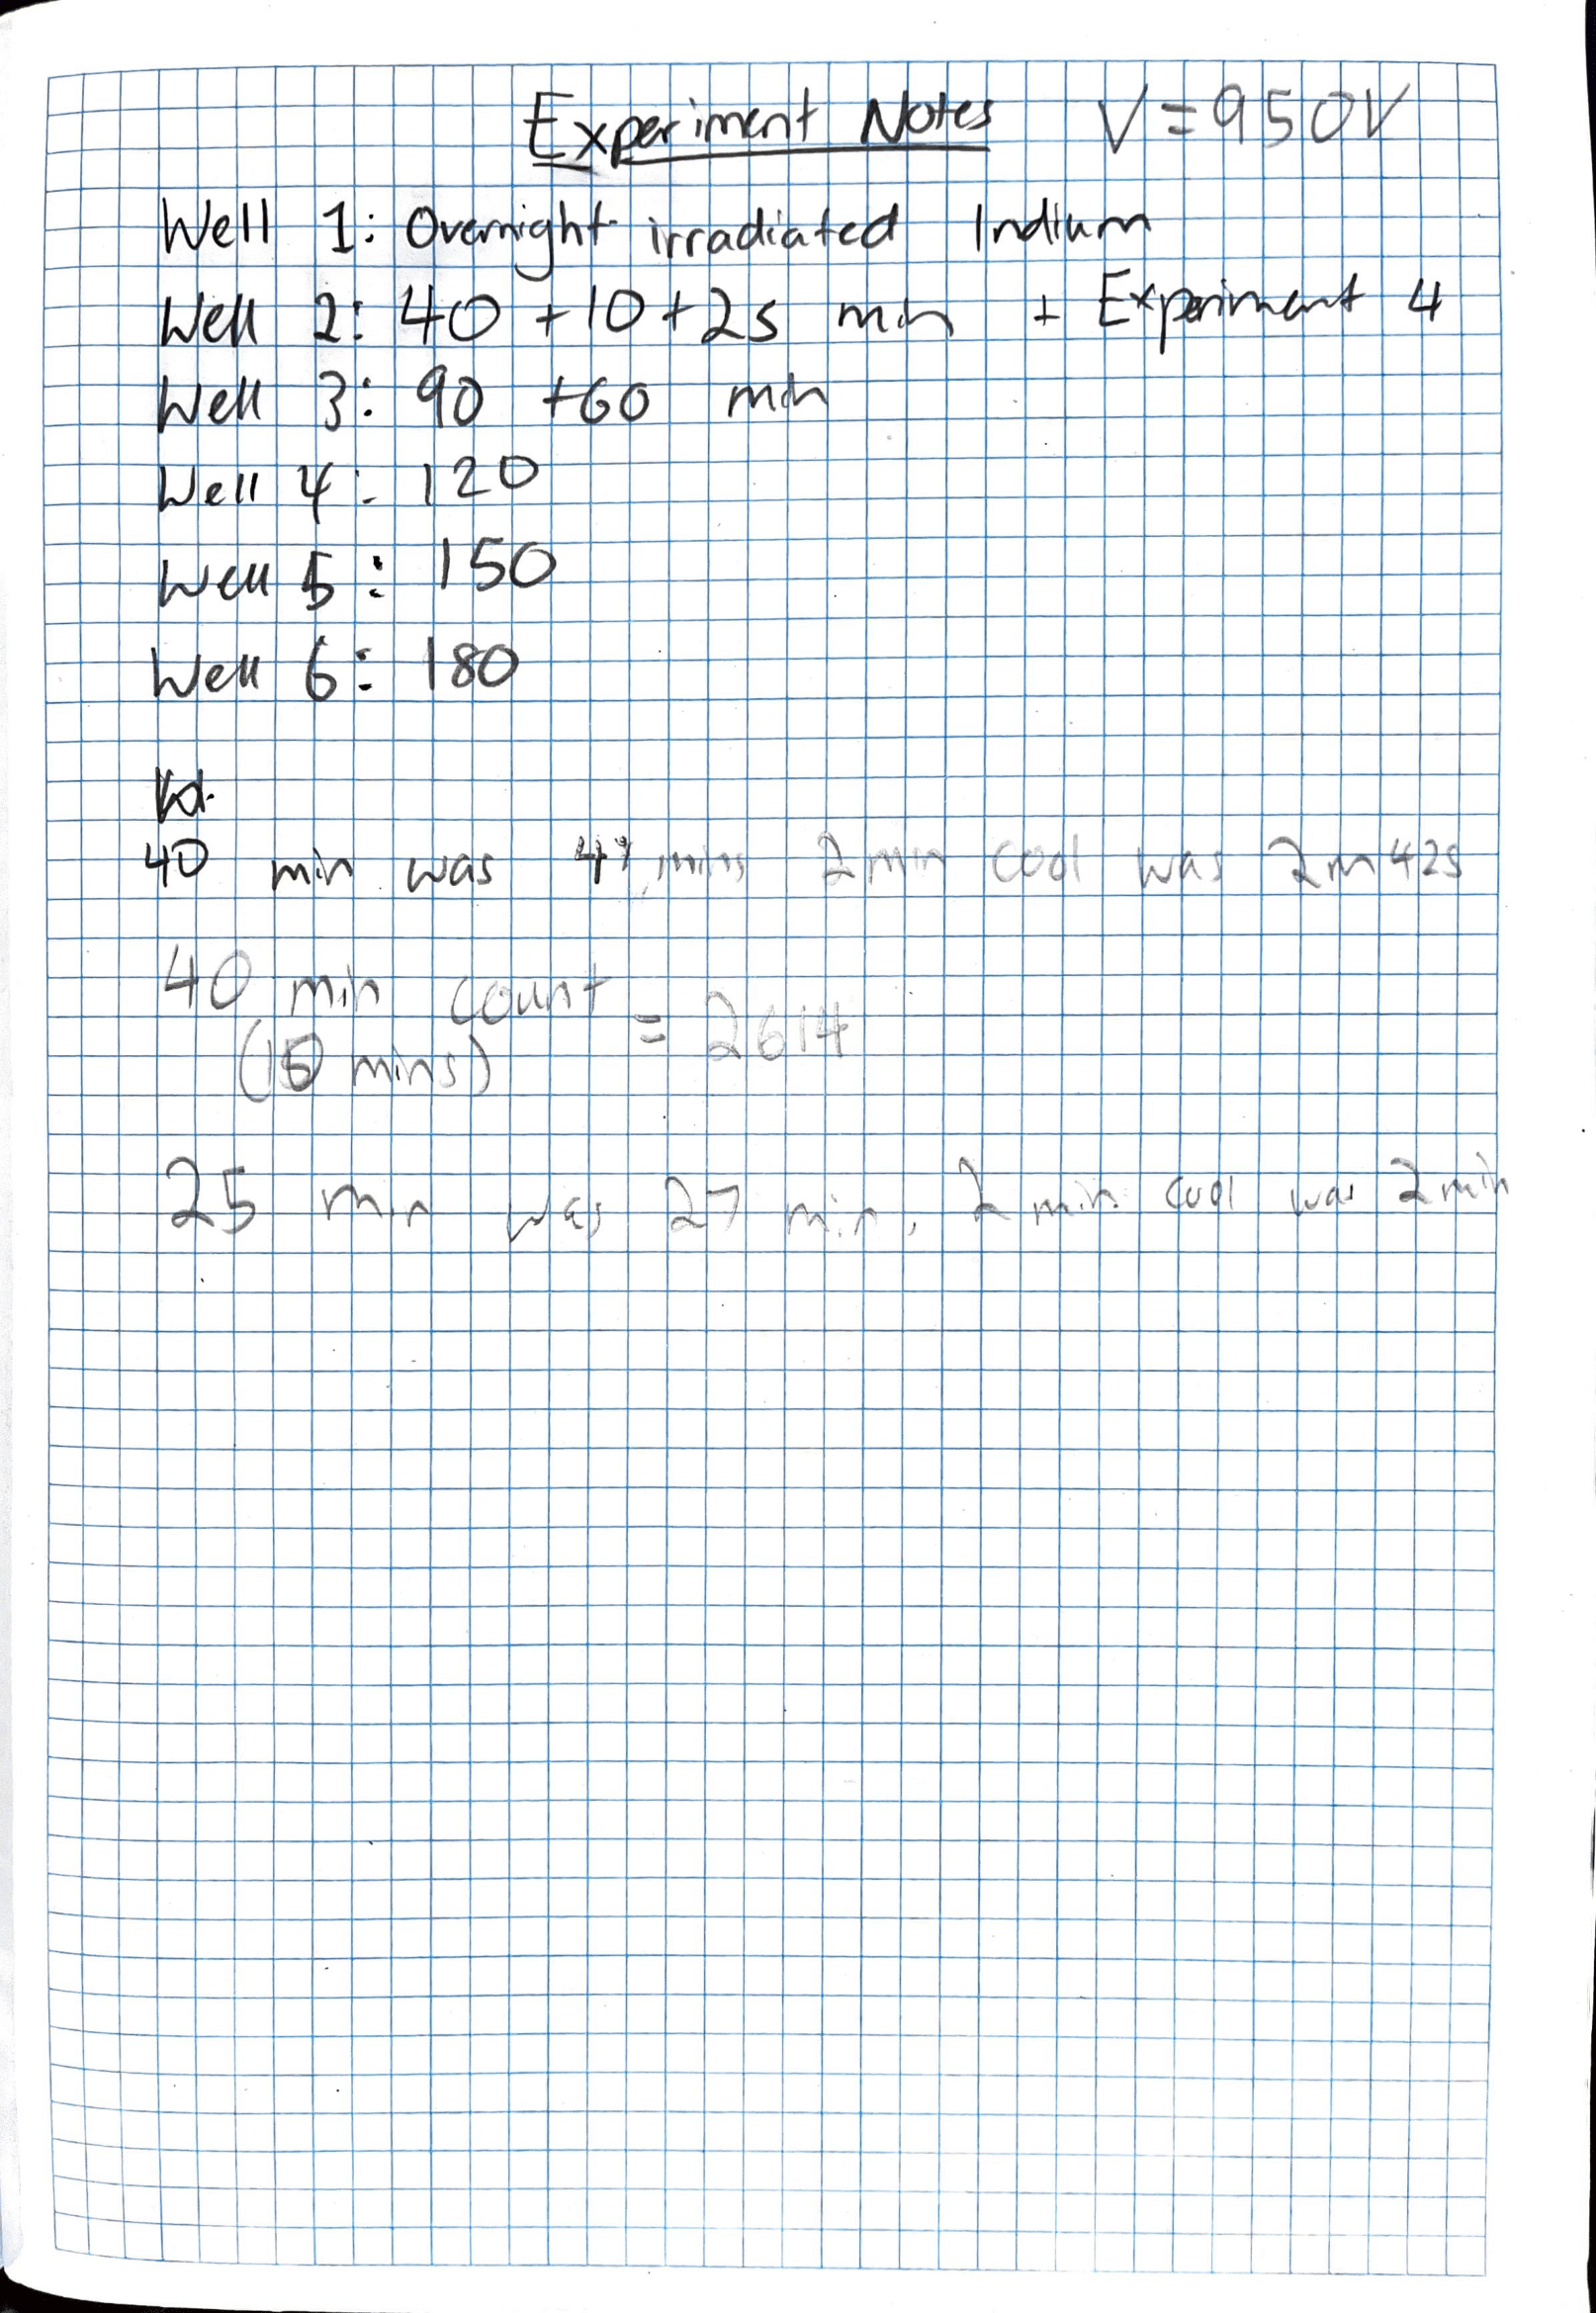
\includegraphics[width=0.8\textwidth]{../Figures/labbook.png}
\end{figure}

\end{document}